% !TeX root = ../main.tex
\chapter{Numerical investigation}
\label{chapt:results}


\section{The fermionic correlator}
To start with the study of the model, we want to analyse the behaviour of the fermionic correlator and illustrate the fermionic masses extraction procedure. \\
Let us initially restrict to $g = 0$, so that the Dirac operator reduces to the one of free Wilson fermions \textcolor{red}{ref eq.}
\raggedright We then compute the correlator numerically via a single inversion of the Dirac operator as detailed in Appendix \ref{chap:AppendixC}. The lattice volume is chosen to be $128 \times 128$. \\
Figure \ref{fig:correlator_mass} reports the fermionic correlator as a function of $m_q$. One can see that a bigger bare quark mass results in a quicker decay, in accordance with the decay law \textcolor{red}{ref. eq.}. On the other side, a smaller mass results in a slower decay and tends to deform the characteristic shape of the correlator. \\~\\
\begin{figure}[h]
    \centering 
    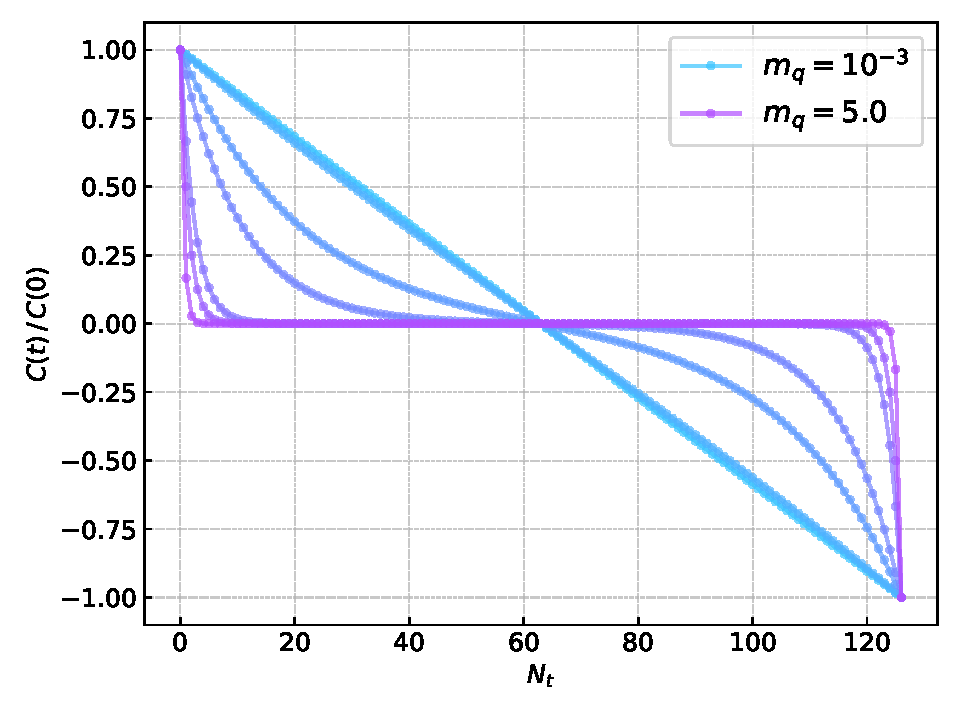
\includegraphics[scale=0.6]{figures/correlator/correlator.pdf}
    \caption[Fermionic correlator]{Normalised fermionic correlator for different values of the bare quark mass. A bigger mass results in a quicker decay, according to \textcolor{red}{eq. ref.}}
    \label{fig:correlator_mass}
\end{figure}
Figure \ref{fig:correlator_CGiter} shows the number of iterations needed for convergence of the Conjugate Gradient algorithm. While the exact number depends on the desired tolerance, one can clearly see that the number of iterations grows as $m_q \to 0$, due to an increase in the condition number \cite{cond_num_ref}. \\
\begin{figure}[h]
    \centering 
    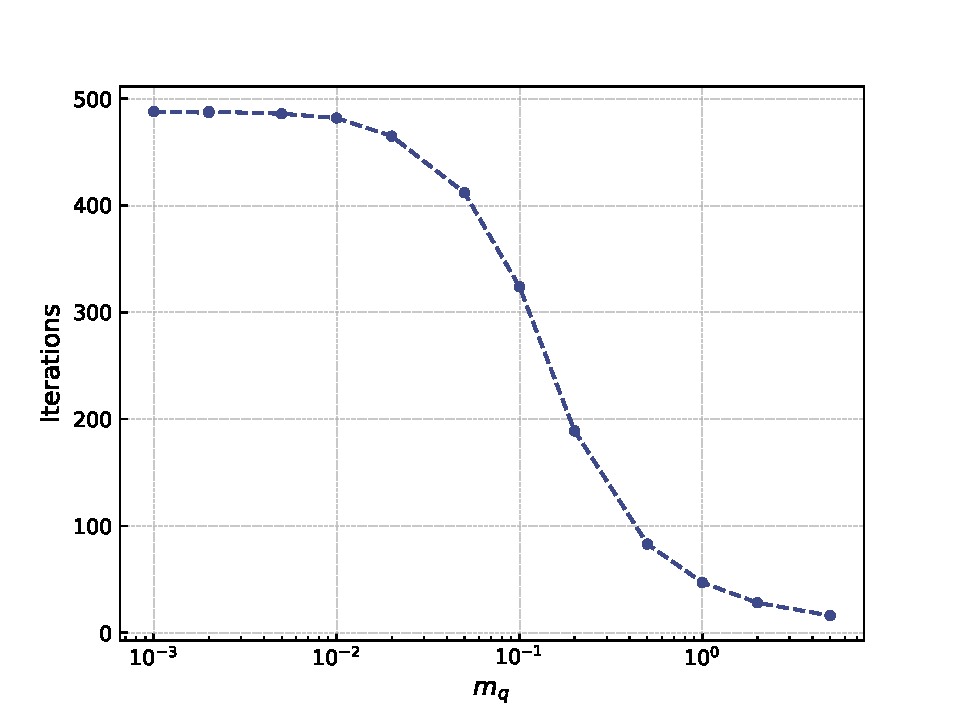
\includegraphics[scale=0.6]{figures/correlator/CGiter.pdf}
    \caption{CG iterations}
    \label{fig:correlator_CGiter}
\end{figure} 
\newpage
For the Dirac operator \textcolor{red}{ref eq.}, one can derive an analytical expression for the fermionic mass. The Dirac operator in momentum space reads \textcolor{red}{non lo hai mai introdotto}
\begin{equation*}
\bar{D}(p)= m_q + \sum_\mu 2 \sin ^2\left(\frac{p_\mu}{2}\right)+i \sum_\mu \gamma_\mu \sin \left(p_\mu\right)
\end{equation*}
and its inverse is
\begin{equation*}
    \bar{D}^{-1}(p) = \frac{m_q + \sum_\mu 2 \sin ^2\left(\frac{p_\mu}{2}\right) - i \sum_\mu \gamma_\mu \sin \left(p_\mu\right)}{m_q + \sum_\mu 2 \sin^2\left(\frac{p_\mu}{2}\right) + \sum_\mu \sin^2 \left(p_\mu\right)}.
\end{equation*}
One can now find the pole by imposing the numerator evaluated at $p^\mu =(im_\text{phys}, 0)$ to zero:
\begin{equation*}
    \left[m_q + \sum_\mu 2 \sin ^2\left(\frac{p_\mu}{2}\right)\right]^2_{p_\mu = (im_\text{phys}, 0)} + \left[\sum_\mu \gamma_\mu \sin \left(p_\mu\right)\right]^2_{p_\mu = (im_\text{phys}, 0)} = 0.
\end{equation*}
This results in a trascendental equation 
\begin{equation*}
    \left[m_q - 2 \sinh^2\left(\frac{m_\text{phys}}{2}\right)\right]^2 - \sinh^2\left(m_\text{phys}\right) = 0,
\end{equation*}
which has the solution 
\begin{equation}
    m_\text{phys} = \log\left(1+m_q\right).
    \label{eq:analytical_wilson}
\end{equation}
We then choose three values of the bare quark mass, compute the correlator numerically and perform a fit according to \eqref{eq:correlator_mass_extraction}, in order to extract the physical mass. We then compare it to the theoretical value given by \textcolor{red}{add ref. eq.}. The results are reported in figures \ref{fig:corr_small,fig:corr_medium,fig_corr_big} and table \ref{tab:mass_extraction_free}. \\~\\
\begin{table}
    \centering
    \begin{tabular}[pos]{cccc}
        \toprule 
        $m_q$ & teo & fit & err \\
        \midrule 
        1.0 & 0 & 0.6931537171644739 & 4e-20 \\
        0.1 & 0 & 0.09531020915059212 & 0.004 \\
        0.01 & 0 & 0.009950277657505842 & 0.8 \\
        \bottomrule
    \end{tabular}
    \caption[Fit of the correlator for free Wilson fermions.]{The correlator for free Wilson fermions is fitted to \textcolor{red}{(eqref)} and compared to its analytical value given by \eqref{eq:analytical_wilson}. The precision for the Conjugate Gradient algorithm has been set to $r^2 \leq 10^{-10}$.}
    \label{tab:free_wilson_fit}
\end{table}
\begin{figure}
    \centering
    \begin{subfigure}[b]{0.45\textwidth}
        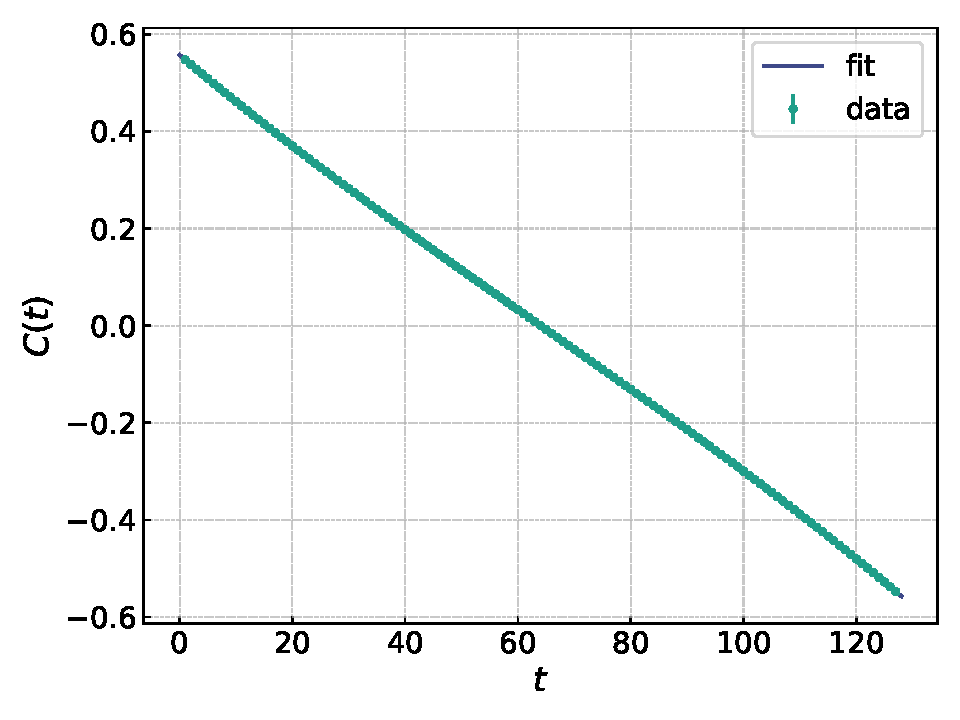
\includegraphics[width=\textwidth]{figures/correlator/corrs_free/corr_small.pdf}
        \caption{$m_q = 0.01$}
    \end{subfigure}
    \hfill
    \begin{subfigure}[b]{0.45\textwidth}
        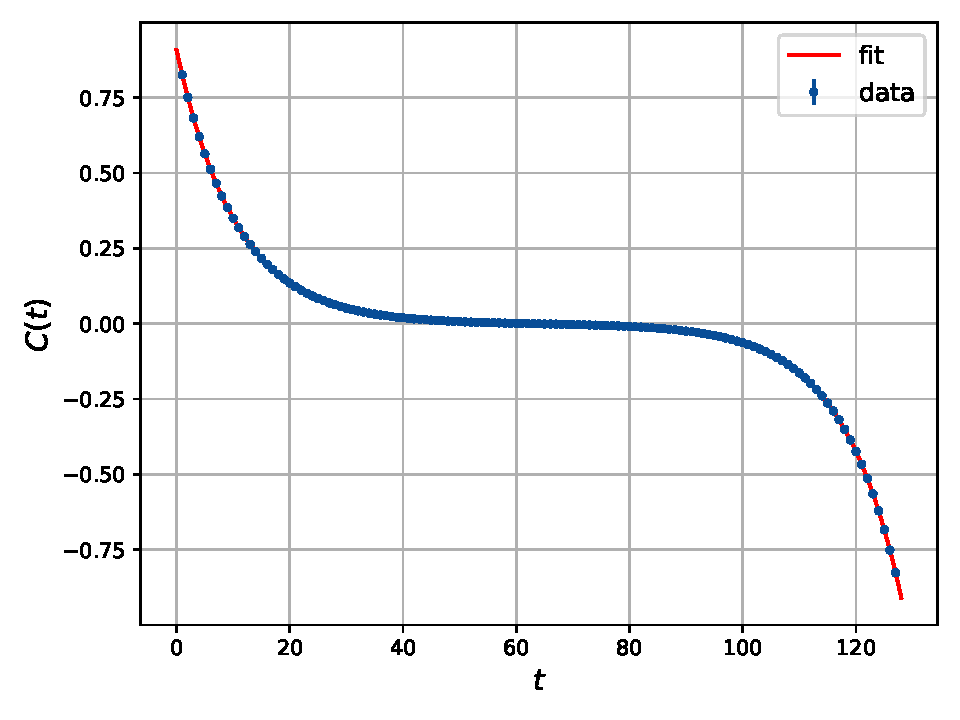
\includegraphics[width=\textwidth]{figures/correlator/corrs_free/corr_medium.pdf}
        \caption{$m_q = 0.1$}        
    \end{subfigure}
    \\
    \vspace{10pt}
    \begin{subfigure}[b]{0.45\textwidth}
        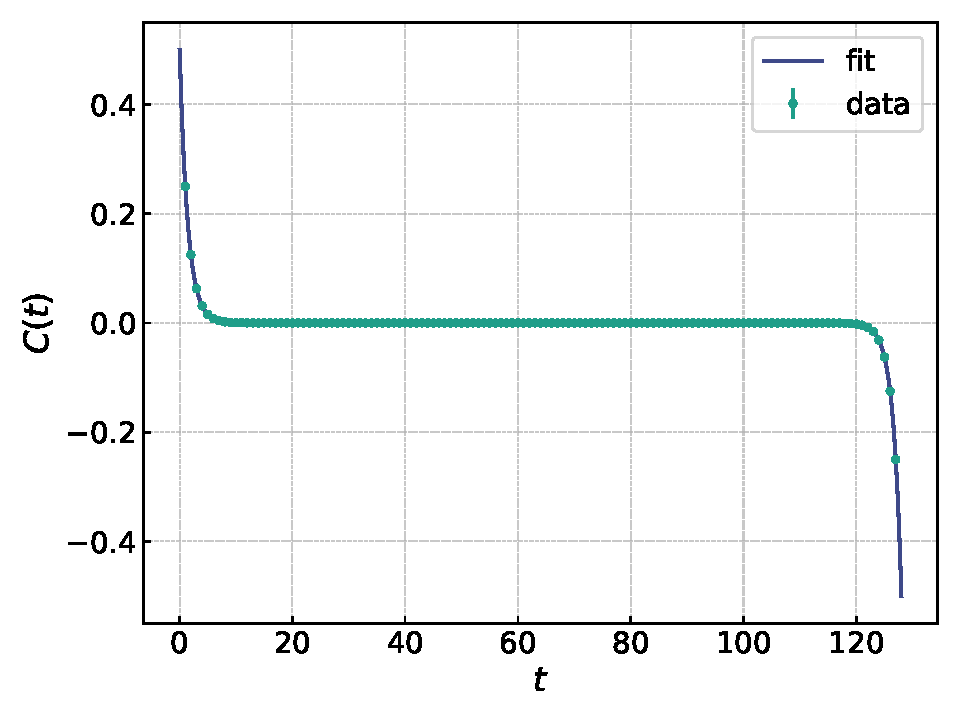
\includegraphics[width=\textwidth]{figures/correlator/corrs_free/corr_big.pdf}
        \caption{$m_q = 1.0$}
    \end{subfigure}
    \caption[Fit of the correlator for free Wilson fermions.]{Fit of the fermionic correlator to \textcolor{red}{(eqref)}, for three different values of the bare quark mass.}
\end{figure}
\textcolor{green}{The presence of a background field has the same effects on the correlator as a bare quark mass. In fact, if $\phi(x) = v$, one can simply redefine the bare mass as $M_q = m_q + g \, v$ and the properties of the fermionic correlator remain unchanged.}
\newpage

\section{Phase diagram}

We want to start the analysis of the Yukawa theory by doing a parameters scan, in order to have a global picture of the phase diagram in the presence of Wilson fermions.
\begin{figure}
    \centering
    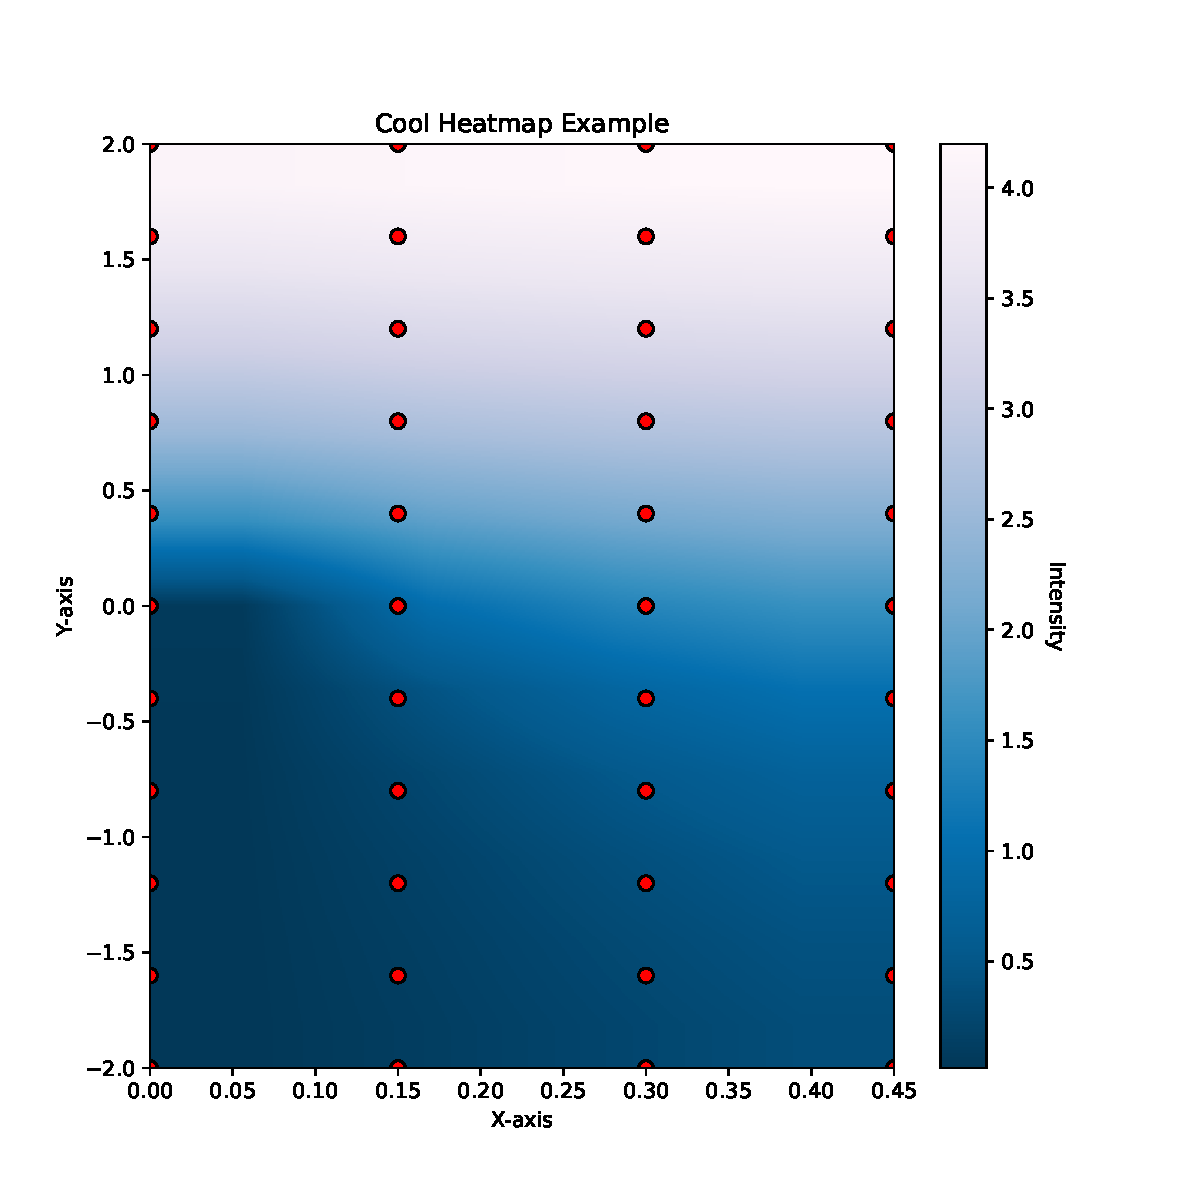
\includegraphics[width=0.7\textwidth]{figures/phase_diagram/phi.pdf}
    \caption{Phase diagram - magnetisation}
    \label{fig:phase_diagram_phi}
\end{figure}

\section{Classical-to-quantum interpolation}

\label{sec:classical_to_quantum}

\begin{figure}
    \centering
    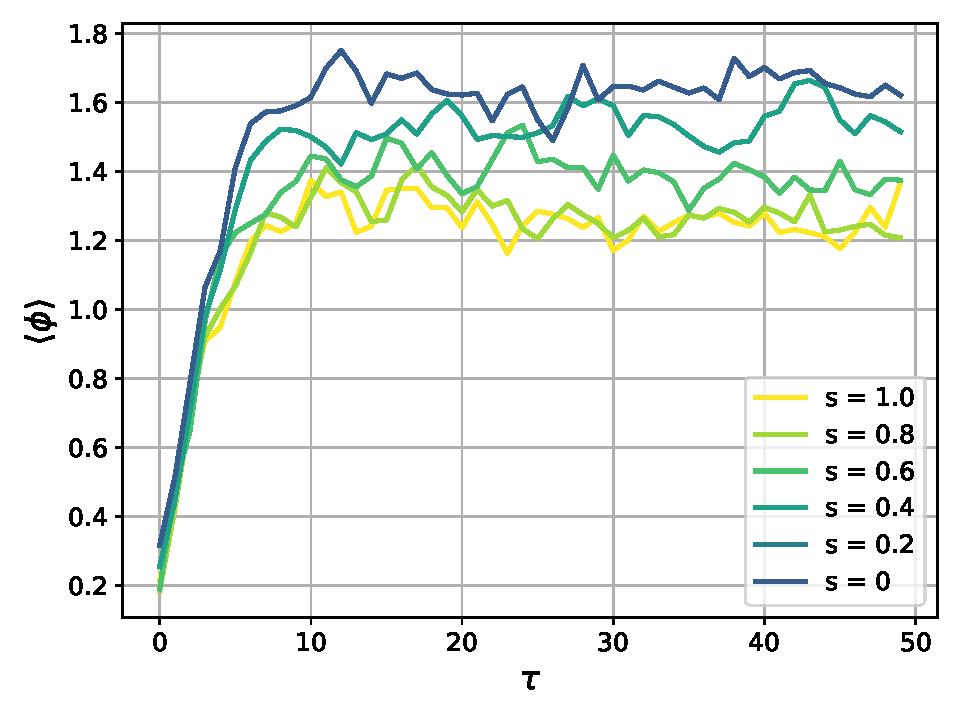
\includegraphics[width=0.7\textwidth]{figures/slide_broken/thermalisation.pdf}
    \caption{}
    \label{fig:thermalisation_different_noise_fracs}
\end{figure}

Let us start by analising the coloured noise field in the simulation and relevant properties that emerge from it. We consider the Yukawa model described by the continuum action \eqref{eq:full_action_continuum} and its discrete vesion \eqref{eq:discretised_action}, \eqref{eq:discretised_effective_action}. \\~\\
Figure \ref{fig:thermalisation_different_noise_fracs} reports the Langevin evolution of the system for different noise fractions. The red line corresponds to the case $s=0$, namely a classical simulation, while the blue line corresponds to the case $s=1$, namely the fully quantum case. 
Note that a lower noise fraction is correlated to a faster convergence towards equilibrium. Moreover, low-distance fluctuations are suppressed due to the removal of the ultraviolet modes in the noise term. \\~\\
We now move on to analyse equilibrium properties. Coloured noise allows for a smooth interpolation between the fully quantum and fully classical picture, with a consequent shift of the expectation values of the observables. Figures \ref{fig:cheneso},\ref{fig:cheneso2} report, respectively, the magnetisation and the chiral condensate as a function of the noise fraction $s$. All the quantities in the classical action, including the coupling constants, are kept fixed while changing $s$.
\textcolor{blue}{Each figure reports two plots corresponding to two different parameter configurations. The COLOR1 line corresponds to a system in the symmetric phase, while the COLOR2 line correspond to the broken phase. The exact parameters for the two configurations are reported under the figure.}
\textcolor{red}{non si puo parlare di fase rotta e simmetrica. inoltre commenta sulla relazione phi, psibarpsi con lambda=0. sarebbe bello misurare phi3 in funzione di s e verificare la relation full col condensato}.
\begin{figure}
    \centering
    \begin{subfigure}[b]{0.45\textwidth}
        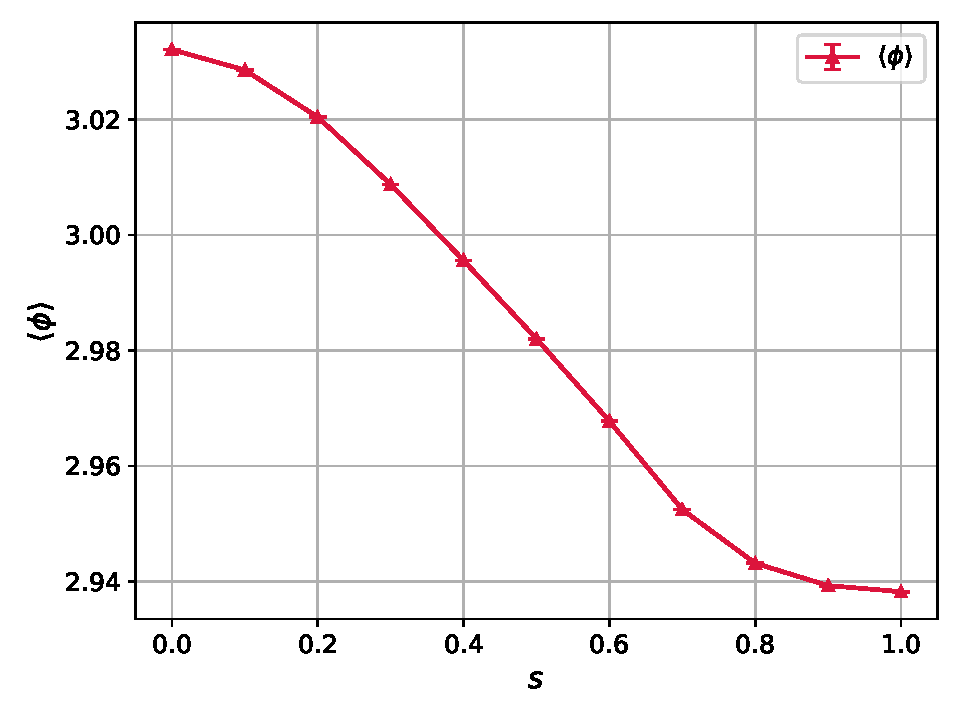
\includegraphics[width=\textwidth]{figures/slide_broken/magnetisation.pdf}
        \caption{Magnetisatoin}
    \end{subfigure}
    \begin{subfigure}[b]{0.45\textwidth}
        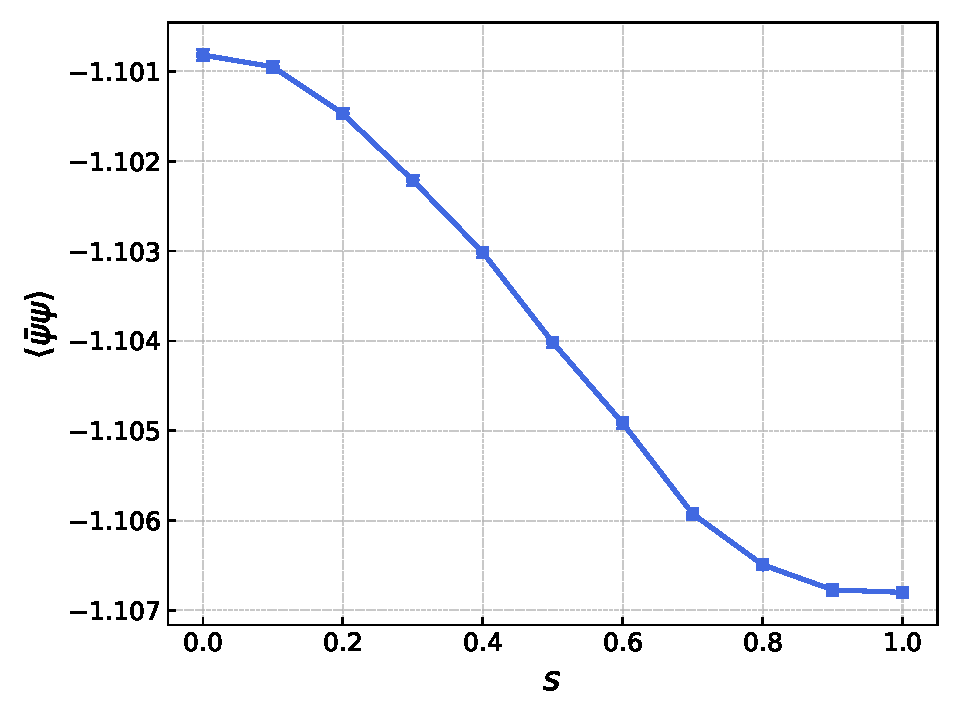
\includegraphics[width=\textwidth]{figures/slide_broken/condensate.pdf}
        \caption{Chiral condensate}
    \end{subfigure}
    \begin{subfigure}[b]{0.45\textwidth}
        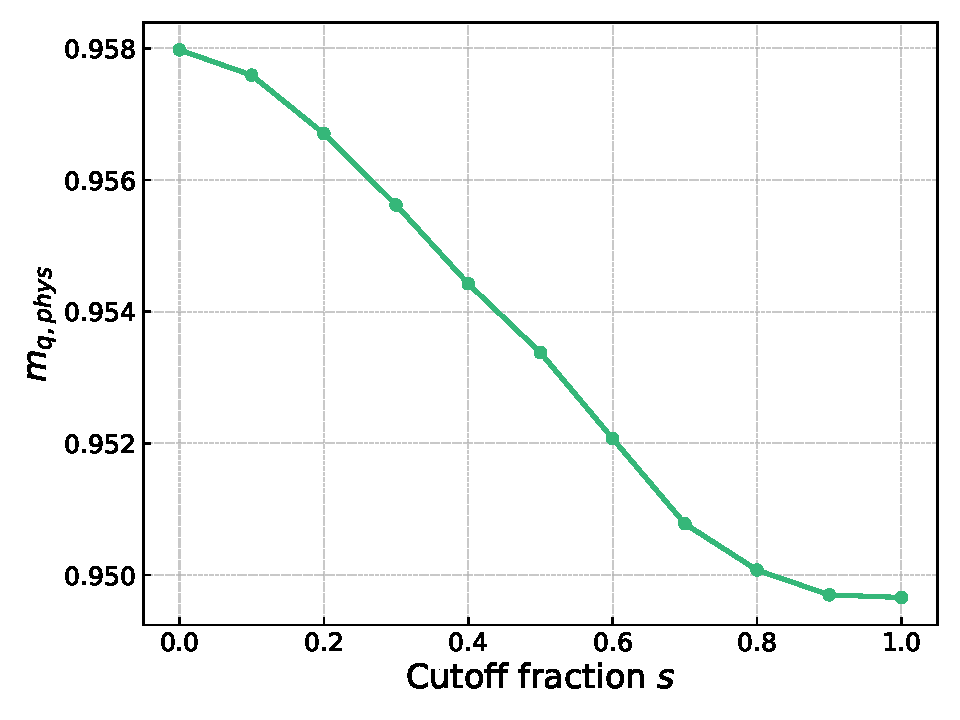
\includegraphics[width=\textwidth]{figures/slide_broken/mass.pdf}
        \caption{Quark mass}
    \end{subfigure}
    \caption[Relation between magnetisation, condensate and mass]{Qualitative relation between magnetisation, chiral condensate and mass, which was motivated in section \ref{sec:Yukawa_theory}. The relation holds at all levels in the quantum theory.}
    \label{fig:interpolation_relation_phi_cond_mass}
\end{figure}
\newpage

\section{Cooling with coloured noise}
Let us now consider one of the main applications of coloured noise, namely the cooling technique. \\
We first set up a white noise simulation $s=1$, and then progressively lower $s$, accomodating the lowering of the cutoff by a change in the couplings, as explained in section  which was described in section \ref{sec:lattice_with_coloured_noise}, and summarised in table \ref{tab:params_cooling}.
\begin{table}[htp]
    \centering
    \begin{tabular}{cccccccc}
        \toprule
        $s$ & $N_t$ & $N_x$ & $m_\phi^2$ & $\lambda$ & $g$ & $m_q$& $K_\psi$ \\
        \midrule 
        1 & 16 & 16 & $m_\phi^2$ & 0.4 & 0.3 & $0.5$ & $K_\psi$ \\
        1/2 & 32 & 32 & $m_\phi^2/4$ & 0.1 & 0.3 & $0.5$ & $K_\psi/4$ \\
        1/4 & 64 & 64 & $m_\phi^2/16$ & 0.025 & 0.3 & $0.5$ & $K_\psi/16$ \\
        1/8 & 128 & 128 & $m_\phi^2/64$ & 0.00625 & 0.3 & $0.5$ & $K_\psi/64$ \\
        \bottomrule
    \end{tabular}
    \caption[Parameters cooling]{Parameters setting in the cooling procedure. Each coupling in the bosonic action is rescaled according to its canonical dimension, while the fermionic sector rescaling is implemented directly at the drift level, as detailed in section \ref{sec:lattice_with_coloured_noise}}.
    \label{tab:params_cooling}
\end{table}
Figure \ref{fig:cooling_M_psibarpsi_chi2} reports the magnetisation, its susceptibility and the chiral condensate as a function of the bare scalar mass $m_\phi^2$. As one can see, there is a general good agreement among the various curves, even with a simple tree-level rescaling.
\begin{figure}[hbp]
    \centering
    \begin{subfigure}[b]{0.45\textwidth}
        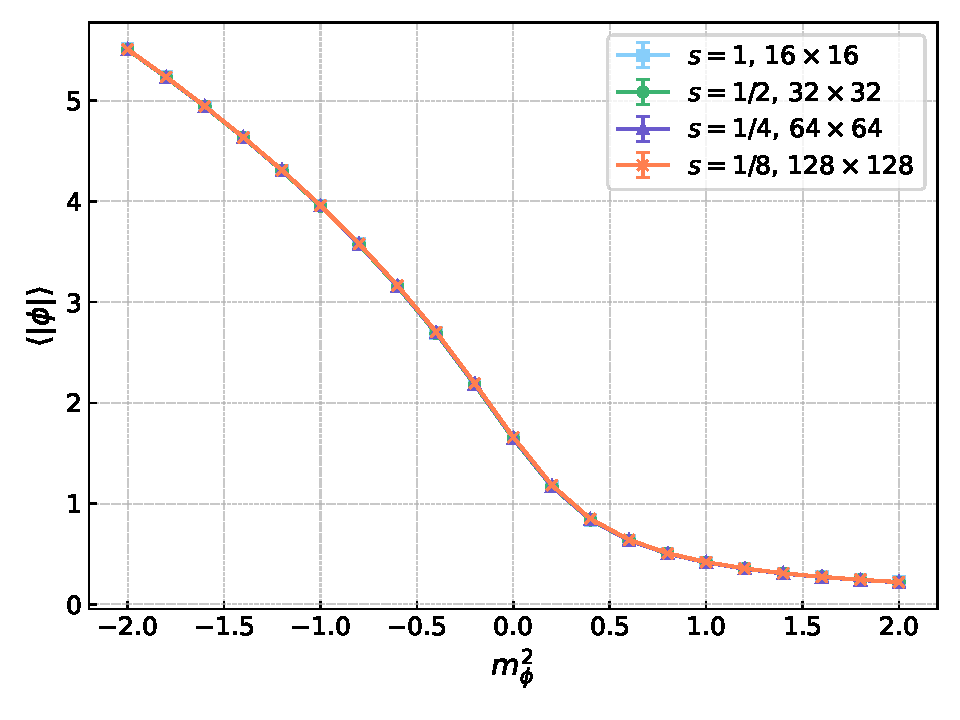
\includegraphics[width=\textwidth]{figures/cooling/mass_scan/magnetisation.pdf}
        \caption{Magnetisation}
    \end{subfigure}
    \hfill
    \begin{subfigure}[b]{0.45\textwidth}
        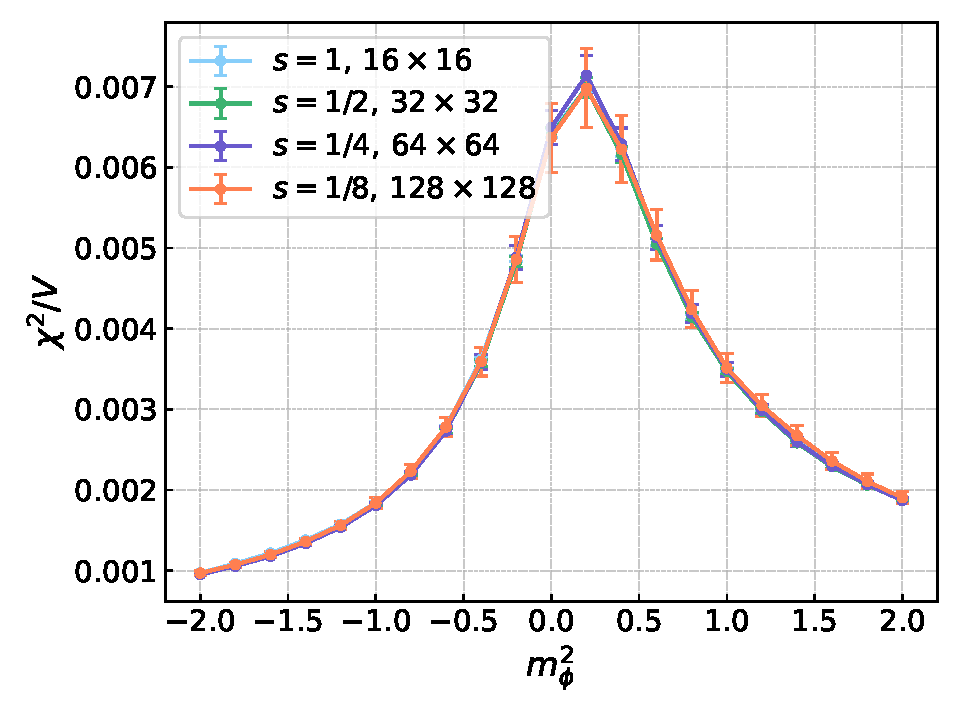
\includegraphics[width=\textwidth]{figures/cooling/mass_scan/susceptibility.pdf}
        \caption{Magnetic susceptibility}
    \end{subfigure}
    \\
    \vspace{10pt}
    \begin{subfigure}[b]{0.45\textwidth}
        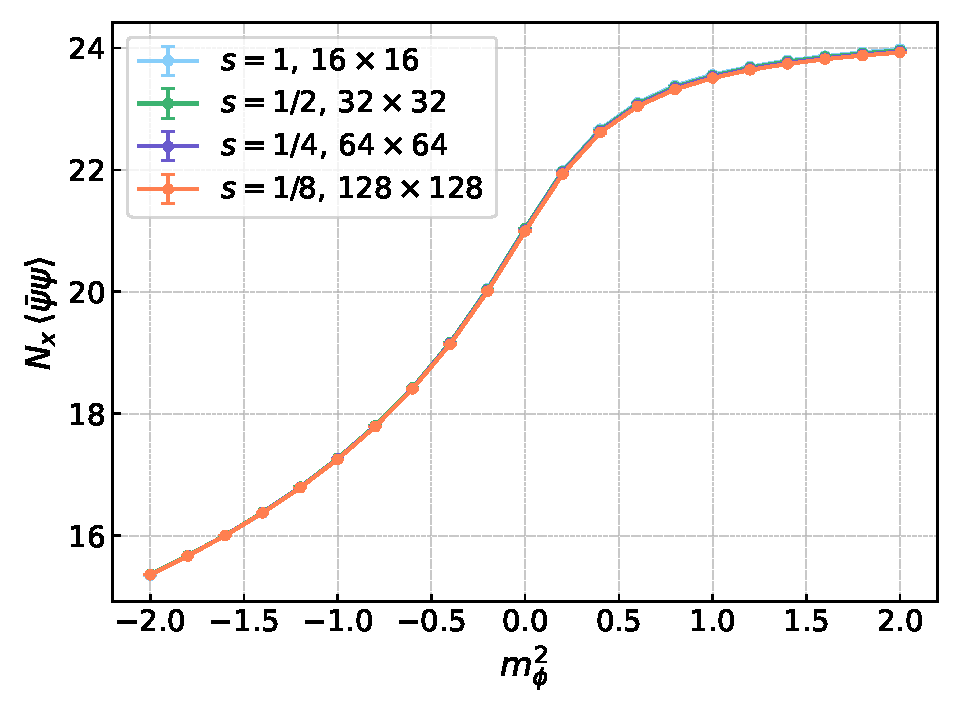
\includegraphics[width=\textwidth]{figures/cooling/mass_scan/condensate.pdf}
        \caption{Chiral condensate}
    \end{subfigure}
    \caption{Overall Caption for the Figure line1 \\ line 2}
    \label{fig:cooling_M_psibarpsi_chi2}
\end{figure}\\
A quantitative comparison for the magnetisation is reported in figure \ref{fig:cooling_deviation}, where we report the relative errors
\begin{equation}
    \begin{aligned}
        \epsilon_\phi(s) &= \frac{\expect{|M|}_{s} - \expect{|M|}}{\expect{|M|}}, \\
        \epsilon_\psi(s) &= \frac{\expect{|\bar\psi \, \psi|}_{s} - \expect{|\bar\psi \, \psi||}}{\expect{|\bar\psi \, \psi||}}.
    \end{aligned}
    \label{eq:cooling_relative_deviation}
\end{equation}
\begin{figure}[htp]
    \centering
    \begin{subfigure}[b]{0.45\textwidth}
        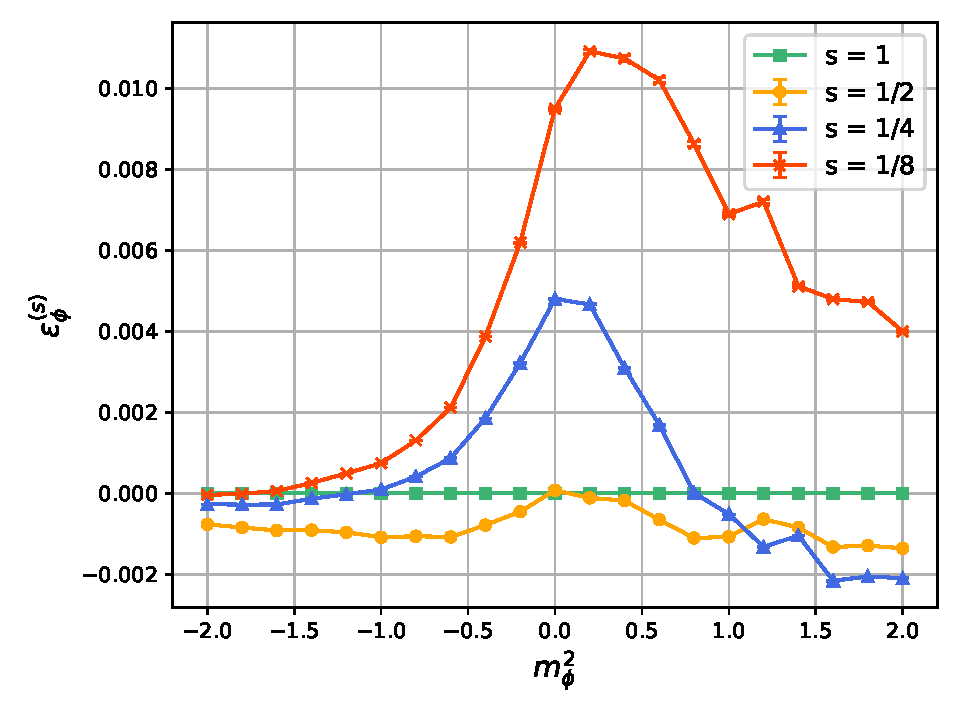
\includegraphics[width=\textwidth]{figures/cooling/mass_scan/deviation.pdf}
        \caption{Absolute magnetisation}
    \end{subfigure}
    \begin{subfigure}[b]{0.45\textwidth}
        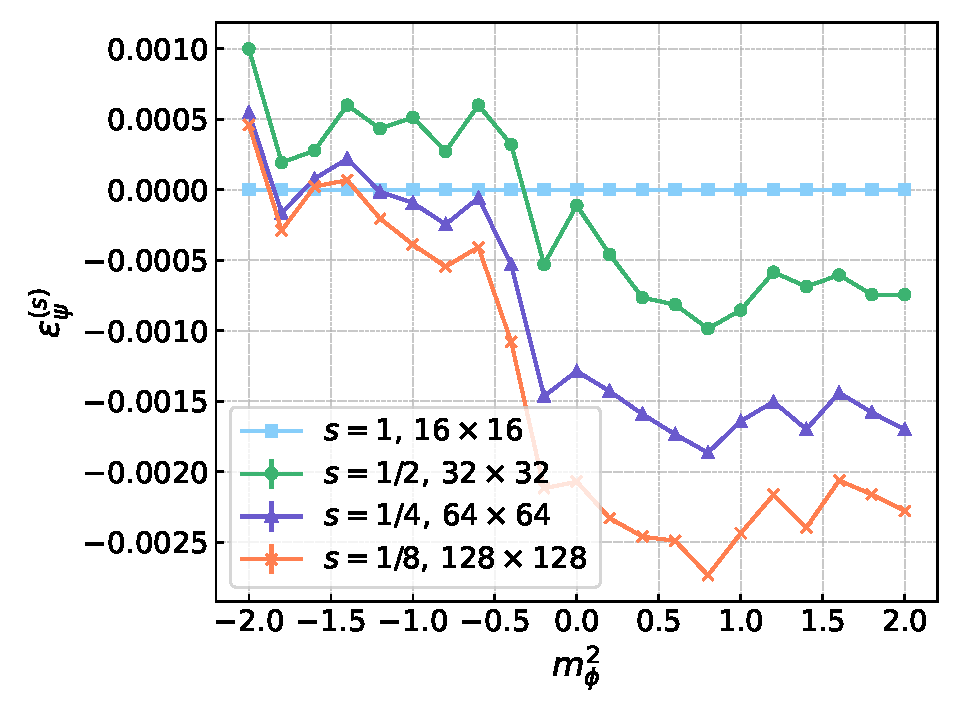
\includegraphics[width=\textwidth]{figures/cooling/mass_scan/deviation_cond.pdf}
        \caption{Chiral condensate}
    \end{subfigure}
    \caption[Relative error in the cooling procedure at tree level.]{Relative error of the absolute magnetisation and chiral condensate in the cooling procedure for various values of the noise fraction $s$.}
    \label{fig:cooling_deviation}
\end{figure}\\
Finally, we want to study some more complex observables such as the fermionic physical mass and the bosonic renormalised mass. They are reported in figure \ref{fig:cooling_masses}. As one can see, there is a clear deviation for $m_{\phi, r}$ at the third block-spin iteration. This is a systematic deviation because \textcolor{red}{i would say tree level, but I don't think it's the case.}
\begin{figure}[hbp]
    \begin{minipage}{0.45\textwidth}
        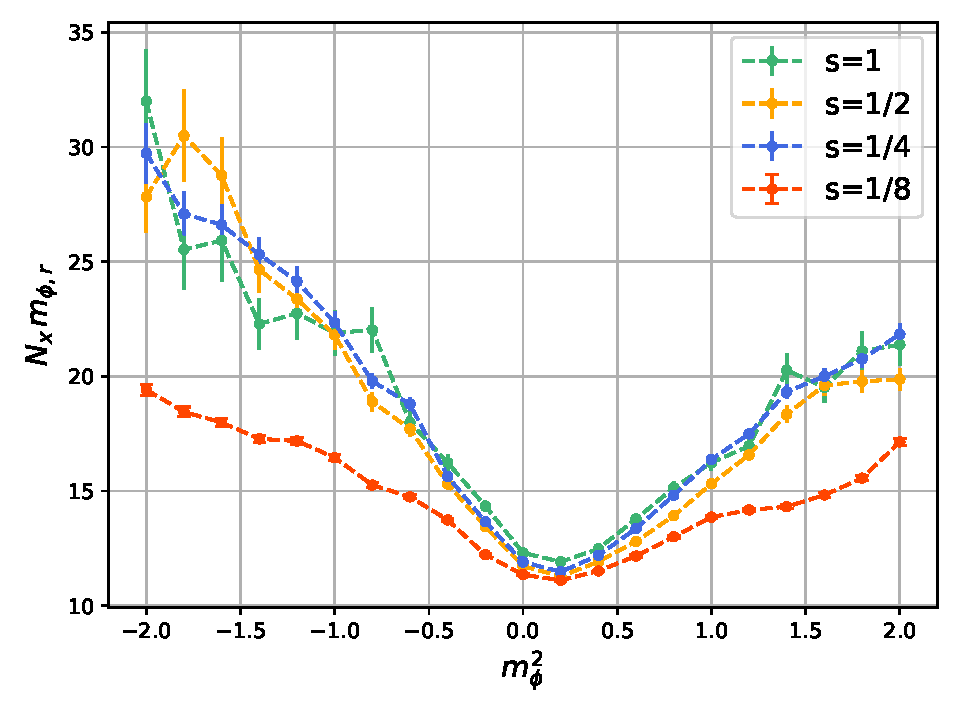
\includegraphics[scale=0.45]{figures/cooling/mass_scan/mphir.pdf}
    \end{minipage}
    \hfill 
    \begin{minipage}{0.45\textwidth}
        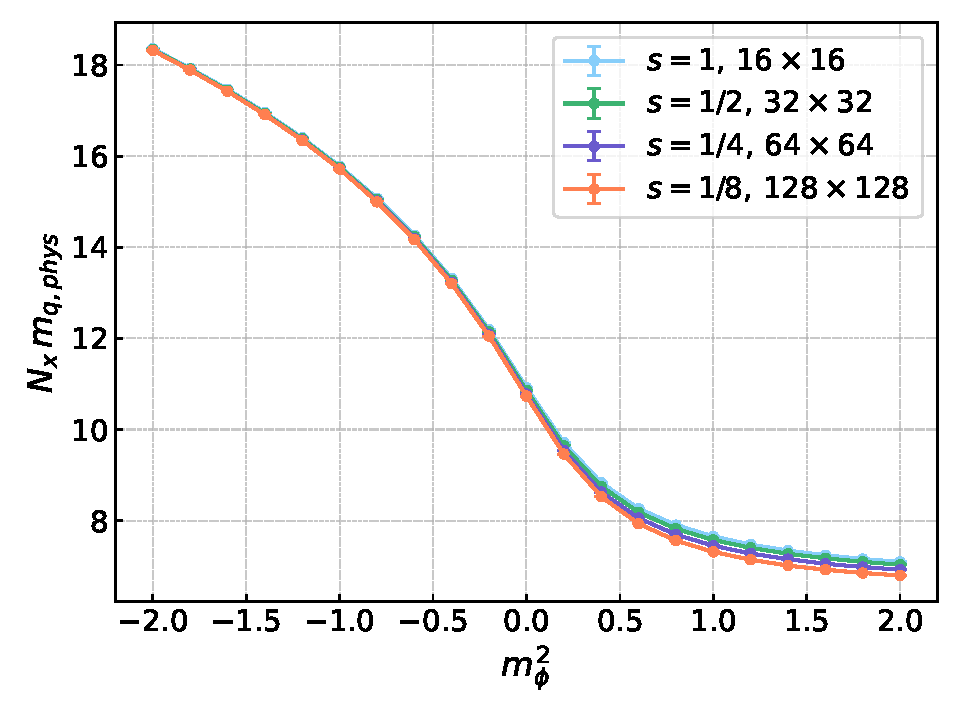
\includegraphics[scale=0.45]{figures/cooling/mass_scan/mqphys.pdf}
    \end{minipage}
    \caption[Masses in the cooling procedure]{Renormalised bosonic mass $m_{\phi, r}$ and pole fermionic mass $m_{q,\text{phys}}$ for various values of the noise fraction $s$.}
    \label{fig:cooling_masses}
\end{figure}


\newpage



\newpage
\section{Chiral fermions and noise-induced chiral phase transition}
\label{sec:chiral_PT}
\textcolor{red}{ricordati di commentare la differenza di scale, giustificazione sfanculata}

\cite{Iwasaki:1994gq}
As explained in section \ref{sec:Yukawa_theory}, chiral symmetry can be broken, in the continumm theory, either explicitly via the introduction of a finite bare quark mass, or spontaneously if the field gains a non-zero expectation value.\\
Moreoveor, in the discrete formulation, the introduction of the Wilson term contributes to the explicit breaking of chiral symmetry, as shown in appendix \ref{chap:AppendixB}. This, in particular, means that chiral symmetry is explicitly broken also for $m_q \to 0$. Because of this, one needs a new definition of the bare mass $M_q$, which takes into account the Wilson term contribution, such that chiral symmetry is restored in the limit $M_q \to 0$. \\
In a lattice study of a theory suchs as  two-flavours QCD, what one typically does is \cite{rothe_LGT,gattringer_LQCD} the following: the spontaneous breaking of chiral symmetry generates three goldstone massless bosons, the pions. If the bare quark mass is zero, the physical mass of the pions has to be zero, as a consequence of \textcolor{red}{cite theorem}. Hence one can measure the pions mass on the lattice and tune $m_q$ such that it is  always zero. \\
This approach is not feasible in our theory, since it is described by a discrete chiral symmetry. While there are proposals for the definition of a bare quark mass for similar theories in the literature \cite{Iwasaki:1994gq,MAIANI1986265}, such approaches are not followed here, because they are very time taking \textcolor{red}{mention CG?}.  Instead here we just consider na\"ive fermions and take the limit $m_q \to 0$. Due to the doubling problem, this represents a theory with $2N_f = 4$ physical degenerate quarks. \\~\\
In figure \ref{fig:scans_classsical_quantum}, the (absolute) magnetisation and the chiral condensate are studied as a function of the bosonic mass squared, both in the fully quantum and fully classical theory. In the classical theory ($s=0$) the order parameters $\left\langle|\phi|\right\rangle, \left\langle\bar\psi \psi\right\rangle$ are, in absolute value, bigger than in the quantum case ($s=1$).  \textcolor{red}{comment on plots: transition point, values of the couplings, susceptibility}. One can see that as $m_q$ is reduced, the systems shifts from a crossover to a second order phase transition, ahighligthed by the susceptibility $\chi^2$ and the binder parameter $U_L$.
\begin{figure}[h]
    \centering
    \captionsetup[subfigure]{justification=centering}
    \begin{subfigure}[t]{0.45\textwidth}
        \centering
        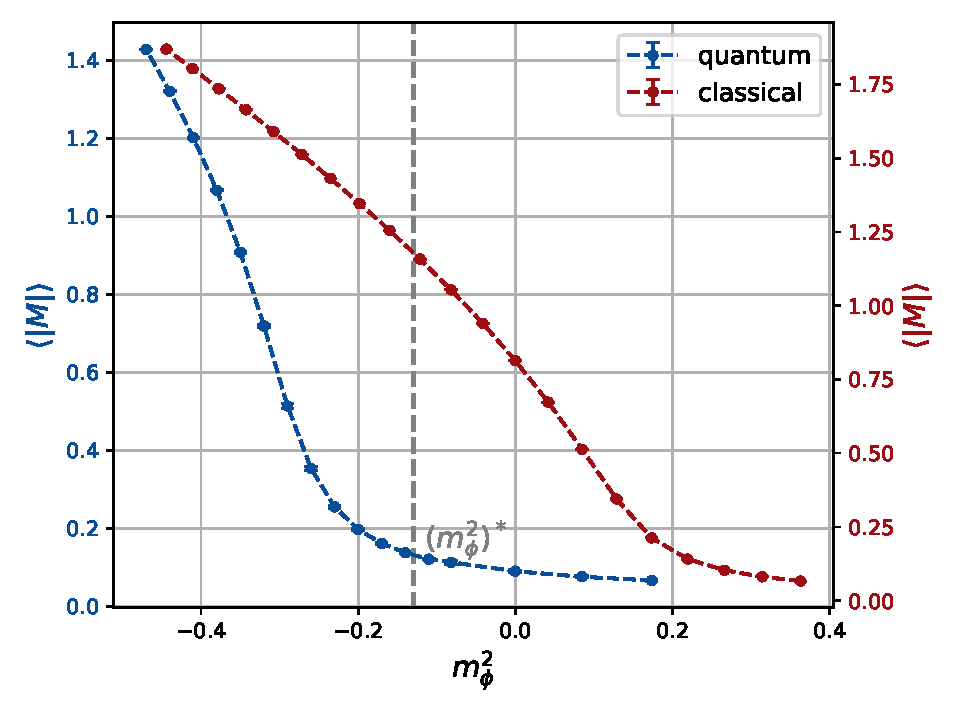
\includegraphics[scale=0.45]{figures/chiral_PT/mass_scan/magnetisation.pdf}
    \end{subfigure}
    \hfill
    \begin{subfigure}[t]{0.45\textwidth}
        \centering
        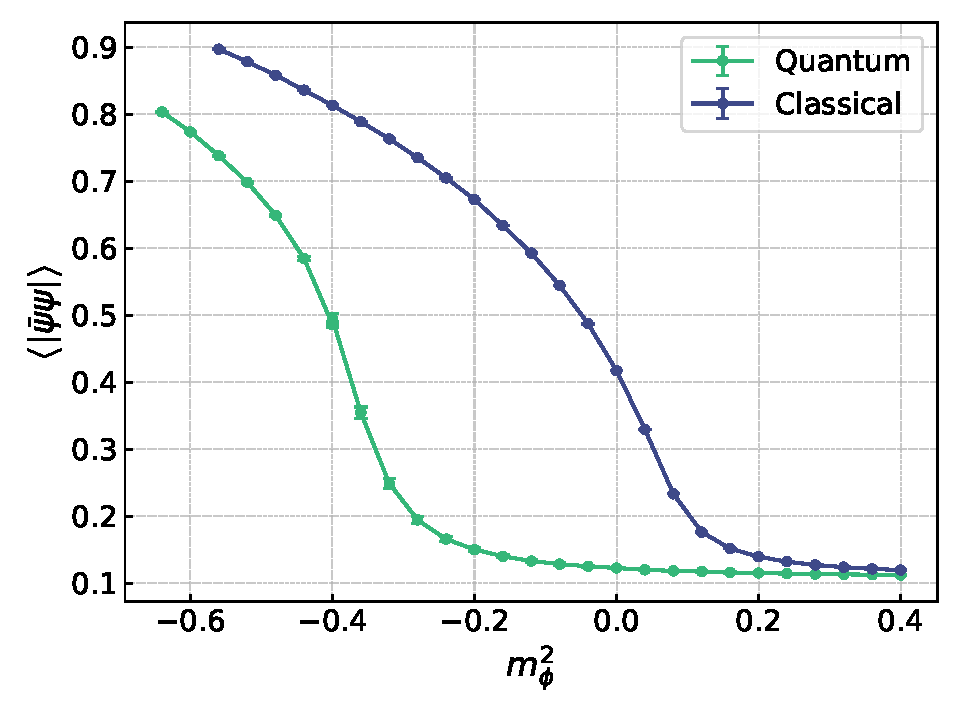
\includegraphics[scale=0.45]{figures/chiral_PT/mass_scan/condensate.pdf}
    \end{subfigure}
    \caption[Mass scan of the quantum and classical theories]{Mass scan of the quantum and classical theories. The dashed gray line indicates a value $m_\phi^{2, \,*}$, where the classical and quantum systems lie in two different phases.}
    \label{fig:scans_classical_quantum}
\end{figure} 

\begin{figure}[h]
\centering
\begin{minipage}{0.45\textwidth}	
	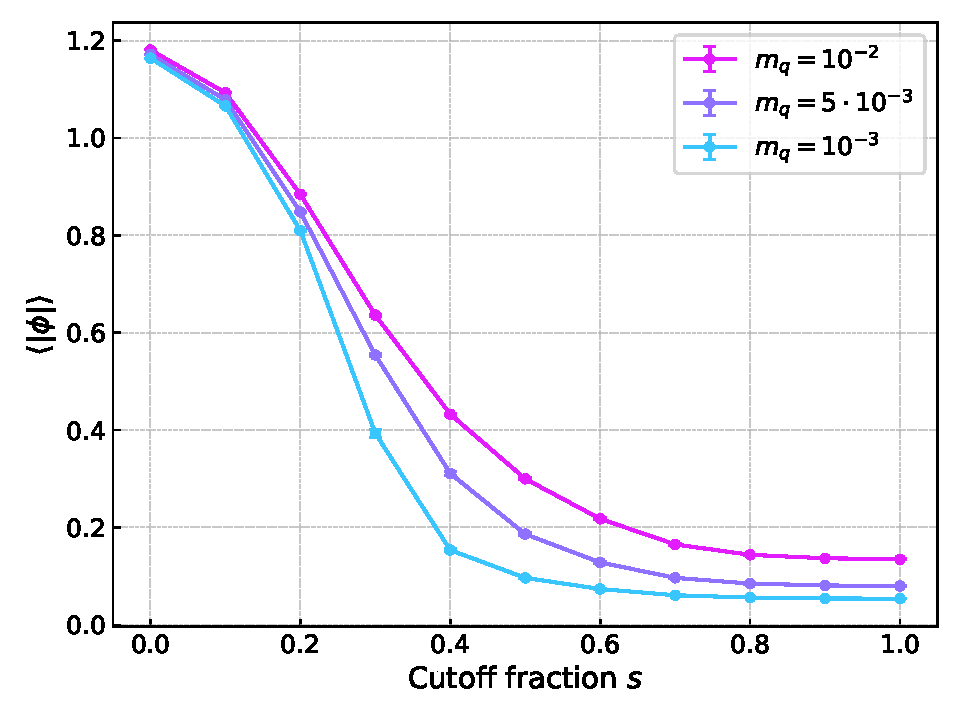
\includegraphics[scale=0.48]{figures/chiral_PT/magnetisation.pdf}
\end{minipage}
\hfill
\begin{minipage}{0.45\textwidth}	
	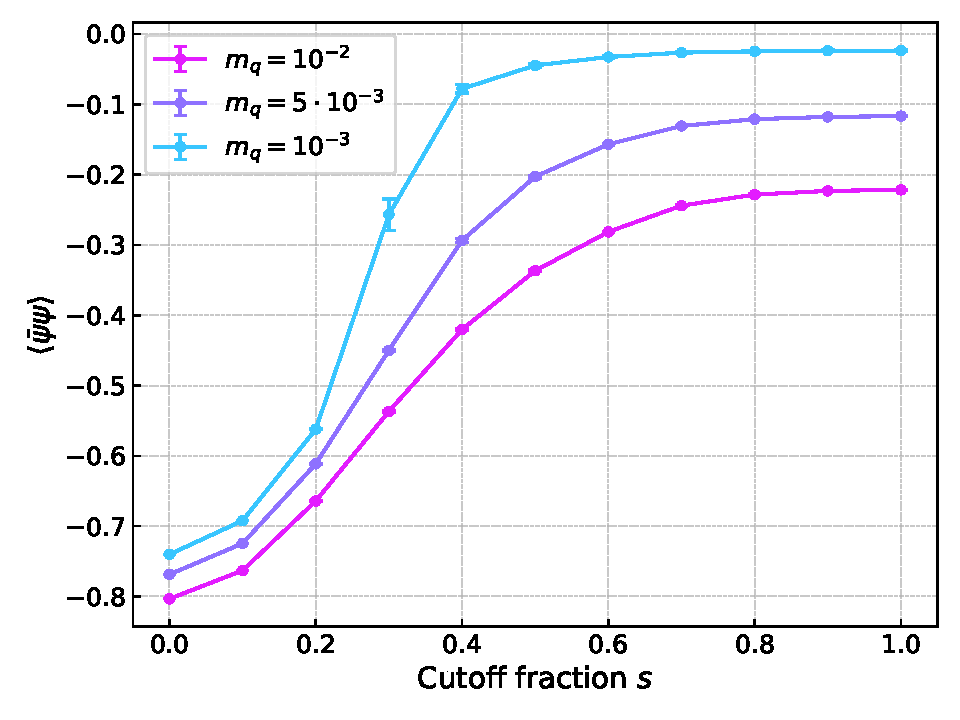
\includegraphics[scale=0.48]{figures/chiral_PT/condensate.pdf}
\end{minipage}
\begin{minipage}{0.45\textwidth}	
	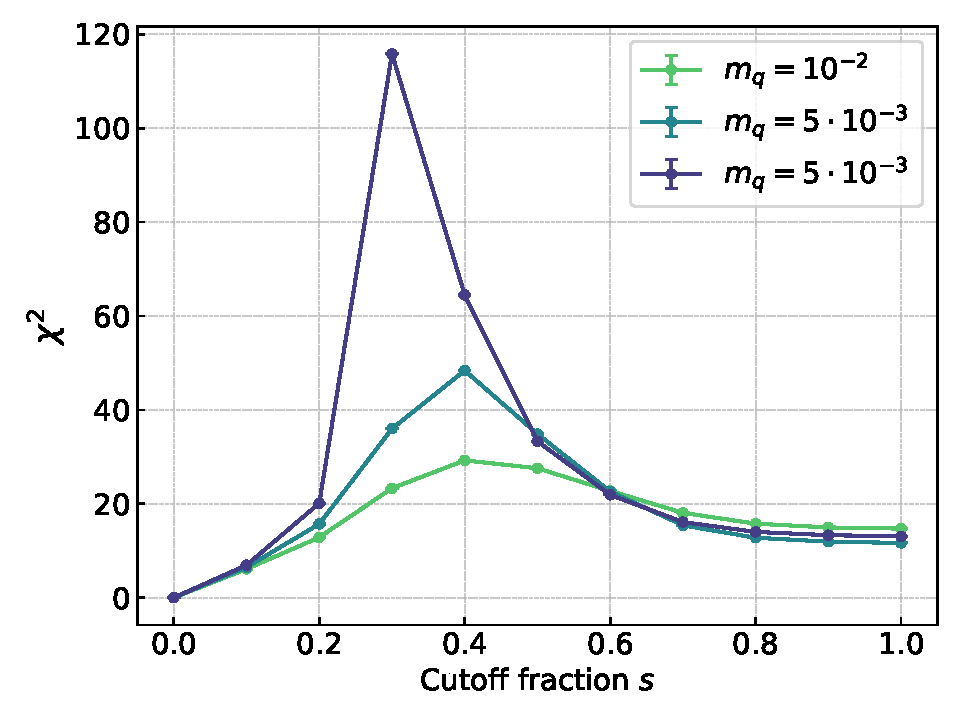
\includegraphics[scale=0.48]{figures/chiral_PT/chi2.pdf}
\end{minipage}
\hfill
\begin{minipage}{0.45\textwidth}
	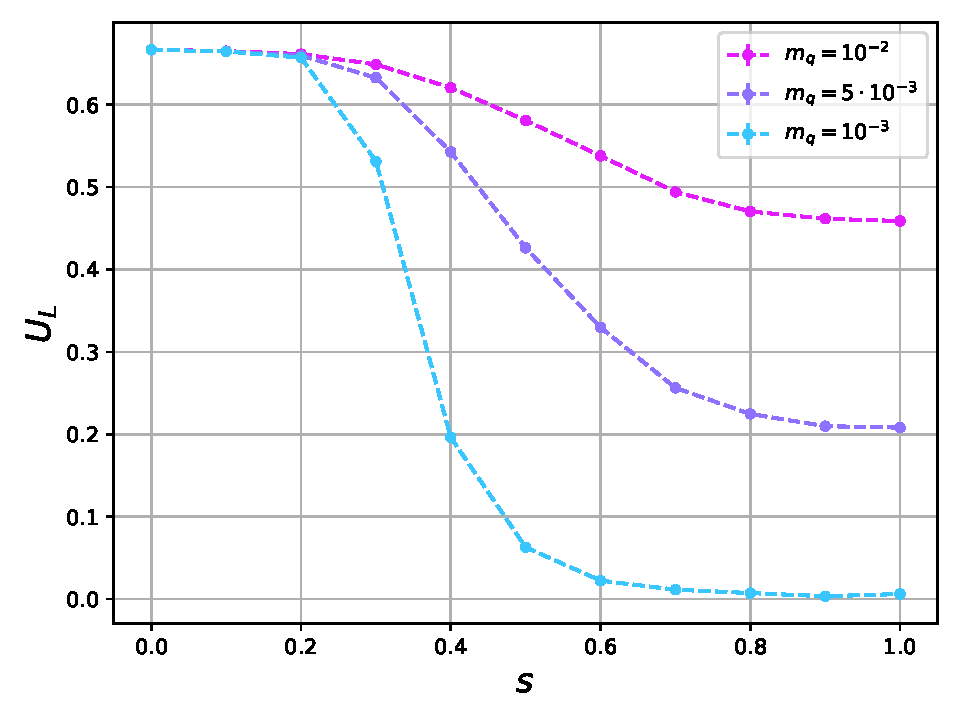
\includegraphics[scale=0.48]{figures/chiral_PT/binder.pdf}
\end{minipage}
\hfill
\caption{Noise-induced phase transition}
\label{fig:chiral:symmetry_breaking}
\end{figure}


